\shorthandoff{>} % desactiva el carácter activo >

\newcommand{\inputnum}{3} 
 
% Hidden layer neurons'number
\newcommand{\hiddennumA}{4}
\newcommand{\hiddennumB}{2}
\newcommand{\hiddennumC}{3}  
 
% Output layer neurons'number
\newcommand{\outputnum}{2} 

 
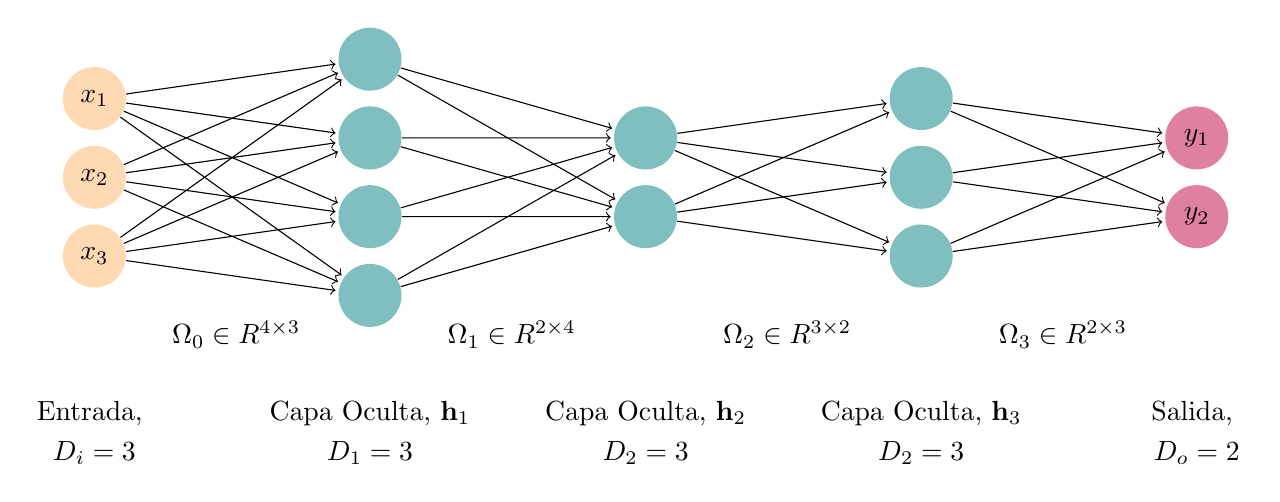
\begin{tikzpicture}
 
% Input Layer
\foreach \i in {1,...,\inputnum}
{
    \node[circle, 
        minimum size = 8mm,
        fill=orange!30] (Input-\i) at (0,-\i) {$x_\i$};
}

\node at (0,-5) {Entrada, $\x$}; 
\node at (0,-5.5) {$D_i = 3$}; 
\node at (1.8,-4) {$\boldsymbol{\Omega}_0 \in \mathbb{R}^{4 \times 3}$}; 






 
% Hidden Layer 1
\foreach \i in {1,...,\hiddennumA}
{
    \node[circle, 
        minimum size = 8mm,
        fill=teal!50,
        yshift=(\hiddennumA-\inputnum)*5 mm
    ] (HiddenA-\i) at (3.5,-\i) {};
}

\node at (3.5,-5) {Capa Oculta, $\mathbf{h}_1$}; 
\node at (3.5,-5.5) {$D_1 = 3$}; 
\node at (5.3,-4) {$\boldsymbol{\Omega}_1 \in \mathbb{R}^{2 \times 4}$}; 





% Hidden Layer 2
\foreach \i in {1,...,\hiddennumB}
{
    \node[circle, 
        minimum size = 8mm,
        fill=teal!50,
        yshift=(\hiddennumB-\inputnum)*5 mm
    ] (HiddenB-\i) at (7,-\i) {};
}

\node at (7,-5) {Capa Oculta, $\mathbf{h}_2$}; 
\node at (7,-5.5) {$D_2 = 3$};
\node at (8.8,-4) {$\boldsymbol{\Omega}_2 \in \mathbb{R}^{3 \times 2}$}; 


% Hidden Layer 3
\foreach \i in {1,...,\hiddennumC}
{
    \node[circle, 
        minimum size = 8mm,
        fill=teal!50,
        yshift=(\hiddennumC-\inputnum)*5 mm
    ] (HiddenC-\i) at (10.5,-\i) {};
}

\node at (10.5,-5) {Capa Oculta, $\mathbf{h}_3$}; 
\node at (10.5,-5.5) {$D_2 = 3$}; 
\node at (12.3,-4) {$\boldsymbol{\Omega}_3 \in \mathbb{R}^{2 \times 3}$}; 

% Output Layer
\foreach \i in {1,...,\outputnum}
{
    \node[circle, 
        minimum size = 8mm,
        fill=purple!50,
        yshift=(\outputnum-\inputnum)*5 mm
    ] (Output-\i) at (14,-\i) {$y_\i$};
}

\node at (14,-5) {Salida, $\y$}; 
\node at (14,-5.5) {$D_o = 2$};

%COONEXION ENTRADA -> CAPA1
\foreach \i in {1,...,\inputnum}
{
    \foreach \j in {1,...,\hiddennumA}
    {
        \draw[->, shorten >=1pt] (Input-\i) -- (HiddenA-\j);   
    }
}


%COONEXION CAPA1 -> CAPA2
\foreach \i in {1,...,\hiddennumA}
{
    \foreach \j in {1,...,\hiddennumB}
    {
        \draw[->, shorten >=1pt] (HiddenA-\i) -- (HiddenB-\j);   
    }
}


%COONEXION CAPA2 -> CAPA3
\foreach \i in {1,...,\hiddennumB}
{
    \foreach \j in {1,...,\hiddennumC}
    {
        \draw[->, shorten >=1pt] (HiddenB-\i) -- (HiddenC-\j);   
    }
}

%COONEXION CAPA3 -> CAPASALIDA
%COONEXION CAPA2 -> CAPA3
\foreach \i in {1,...,\hiddennumC}
{
    \foreach \j in {1,...,\outputnum}
    {
        \draw[->, shorten >=1pt] (HiddenC-\i) -- (Output-\j);   
    }
}

\end{tikzpicture} 


